\documentclass{standalone}
\usepackage{hsbcommon}
\begin{document}
        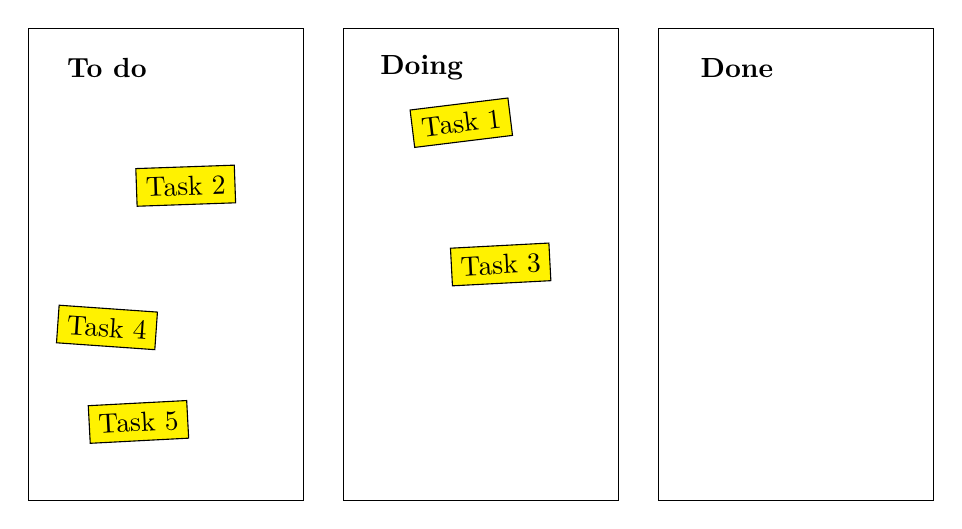
\begin{tikzpicture}
        \draw[draw] (0,0) rectangle (3.5,6);
        \node at (1,5.5) {\textbf{To do}};
        \draw[draw] (4,0) rectangle (7.5,6);
        \node at (5,5.5) {\textbf{Doing}};
        \draw[draw] (8,0) rectangle (11.5,6);
        \node at (9,5.5) {\textbf{Done}};
        \node[draw,fill=yellow,rotate=7] at (5.5,4.8) {Task 1};
        \node[draw,fill=yellow,rotate=2] at (2,4) {Task 2};
        \node[draw,fill=yellow,rotate=3] at (6,3) {Task 3};
        \node[draw,fill=yellow,rotate=-4] at (1,2.2) {Task 4};
        \node[draw,fill=yellow,rotate=3] at (1.4,1) {Task 5};
    \end{tikzpicture}

\end{document}
